% !TeX root = ..\report.tex

\begin{figure}[ht]
    \centering
    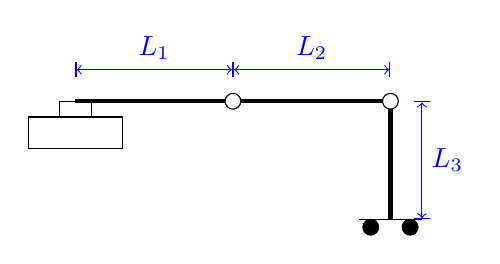
\begin{tikzpicture}
        % Arm 1 and foundation
        \draw (0.6, 0) rectangle (-0.6, -0.4);
        \draw (0.2, 0.2) rectangle (-0.2, 0);
        \draw [ultra thick] (0, 0.2) -- (2, 0.2);

        \begin{scope}[shift={(2,-1.8)}]
            % Arm 2 and joint
            \draw [ultra thick] (0, 2) -- (2, 2);
            \draw [fill=white] (0, 2) circle [radius=0.1];
            
            % Arm 3 and joint
            \draw [ultra thick] (2,2) -- (2,0.5);
            \draw [fill=white] (2,2) circle [radius=0.1];
            \draw (1.6, 0.5) -- (2.4, 0.5);
            \draw [fill=black] (1.75, 0.4) circle [radius=0.1];
            \draw [fill=black] (2.25, 0.4) circle [radius=0.1];
            
            \draw [|<->|, blue] (0, 2.4) -- (2, 2.4) node [pos=0.5, above] {$L_2$};
            \draw [|<->|, blue] (2.4, 2) -- (2.4, 0.5) node [pos=0.5, right] {$L_3$};
        \end{scope}

        \draw [|<->|, blue] (0, 0.6) -- (2, 0.6) node [pos=0.5, above] {$L_1$};
    \end{tikzpicture}
    \caption{机械臂主体部分示意图}
    \label{fig:robotic-arm-schema}
\end{figure}
